% 
%  chapter1.tex
%  ThesisISEL
%  
%  Created by Matilde Pós-de-Mina Pato on 2012/10/09.
%
\chapter{Context and Progress status}
\label{cha:introduction}


This report has the objective of informing the reader, about the current status of the development of the dissertation named \textit{From asynchronous IO to reactive stream pipelines}, that is being written by the student \textit{Diogo Paulo de Oliveira Rodrigues}.

Firstly, to understand the current state of development, it is important to make clear what will be the objective and structure of the document that is being written.

This dissertation aims, in the first place, to make an overview on what tools were historically available to deal with non-blocking IO operations and asynchronous programming in general, and then, indentifying what are the state-of-the-art solutions available today to deal with this problem that are usually supported through asynchronous data pipeline architectures.
After presenting state-of-the-art concepts and technologies, some of these tecnhologies will be then compared in terms of performance through the development of practical benchmark test cases, written in several programming languages widely used today.

Taking in account what was explaining above, the dissertation will aim to have the following main structure: 

\begin{enumerate}
	\item Introduction and motivation
	\item Concepts and State of the art
	\item Test case development and Benchmark results 
	\item Conclusions
\end{enumerate}

Since this report is preliminary, this structure can be slightly changed in the course of the development.

To fullfill the objectives in a desirable timeline, were created several tasks scheduled to be done in a pre-determined time interval. This task can be viewed in the  
next Gant diagram, where its possible to see the completion status of each task as they were in 15 of March:


\begin{figure}[ht]
	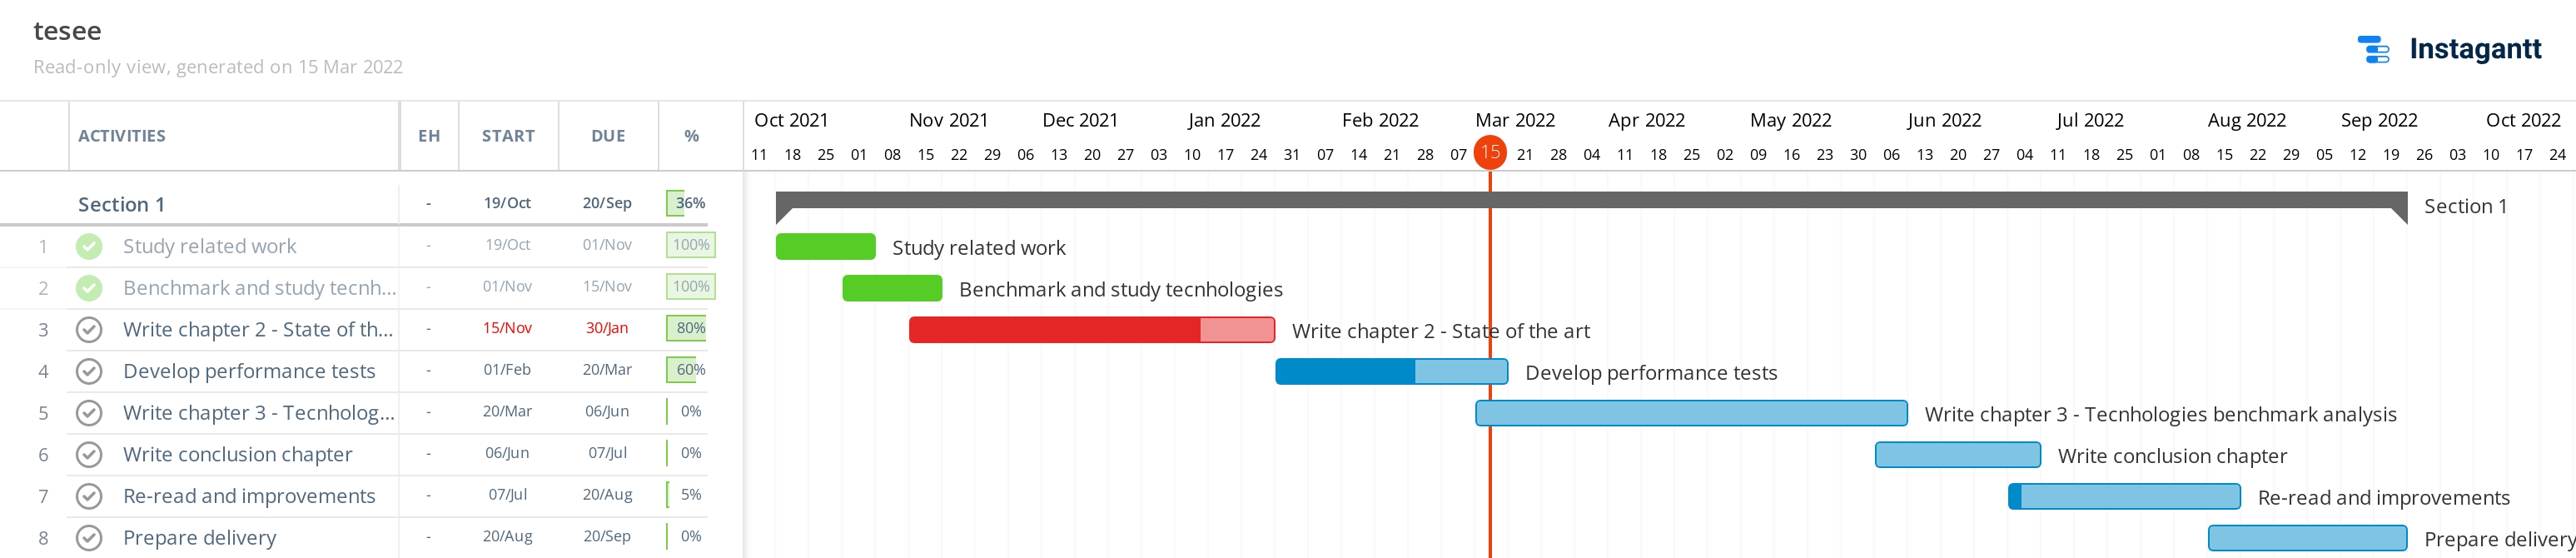
\includegraphics[width=1.20\textwidth]{plan_table}
	  \caption{Planning Gant diagram}
  \label{fig:pla}
\end{figure}

As we can see in the Gant diagram, 80\% of the charpter 2 is completed, however, are remaining some adjustments in some examples and to be more clear in the explanation of others, these adjustments anda complete review will be completed until the final of March.

On the other side, the development of the testing solutions to benchmark the diferent asynchronous pipeline tecnhologies are under course. The finish date to this task is expected to be 20 March, where is expected to begin the writing of the charpter 3 of the thesis.

On the next charpter of this report, is written the charpter 2 of the thesis "\textit{State of the Art}" as it was on the day of 15 of March of 2022.

